\chapter{Simulations and Results}
\label{chap:scenarios} 

This chapter will test the adaptation algorithms implemented in the \textit{ABR}
module from the \autoref{chap:abrmodule} in various simulated scenarios. The \autoref{sec:metrics}
will present the metrics used for the comparisons. The \autoref{sec:scenarios} will 
go through all the simulation scripts and its results. The \autoref{sec:fairness} will
analyse the fairness of the adaptation algorithms. Finally, the \autoref{sec:simconclu},
will discuss the conclusions and limitations of the \textit{ABR} module.

% \section{Introduction}

\section{Comparison Metrics}
\label{sec:metrics}

For the comparison, the metrics introduced in the \autoref{sec:qoemetrics} will be used.
In addition, other metrics will be used that may also be of interest. And they are as follows:

\begin{itemize}[topsep=0pt, noitemsep]
    \item \textbf{Average Throughput}. The average of the network throughput.
    \item \textbf{Playback start time}. The time the client takes to start the playback.
    \item \textbf{Total time watched}. Total time watched by the client.
    \item \textbf{Quality switches}. The number of times the representation changed.
    \item \textbf{Paused times}. The number of times the playback paused.
    \item \textbf{Time at each quality}. The time spent at each quality.
    \item \textbf{Buffer status}. The buffer status in milliseconds of content as a function of time.
    \item \textbf{QoE Score}. This is a score based on various metrics, the formula is as follows:
    \begin{equation}
        QoE\ score = \frac{t_w-pb_s-\sum_{i=1}^{M} \frac{t_i}{2}\cdot (\frac{1}{2}-\frac{i+1}{M})-\frac{1}{2}\cdot (qs+pt)}{simulation\ time}
    \end{equation}
    with
    \begin{itemize}[topsep=0pt, noitemsep]
        \item[$\circ$] $t_w$ 		                            Time watched
        \item[$\circ$] $pb_s$ 		                            Playback start time
        \item[$\circ$] $t_i\ _{q=\{0,1,...,M\}}$ 		        Time at each quality 
        \item[$\circ$] $qs$ 		                            Quality switches
        \item[$\circ$] $pt$ 		                            Paused times
    \end{itemize}
\end{itemize}

\section{Example script}
\label{sec:example}


\section{Scenarios}
\label{sec:scenarios}

In the next sections, the throughput rule of \textit{dash.js} will be refered as \textit{DASH throughput},
the BOLA rule as \textit{BOLA}, the bandwidth estimation of \textit{hls.js} as \textit{HLS} and the combination
of the BOLA and the throughput rule of \textit{dash.js} simply as \textit{DASH}.

\subsection{Scenario 1}
This section will take a look a basic network scenario. To be as simply as possible, the will be 
only two nodes linked with a \texttt{PointToPoint} connection. The simulation time is 50 seconds 
and the datarate will vary in time.

\begin{figure}[]
    \centering
    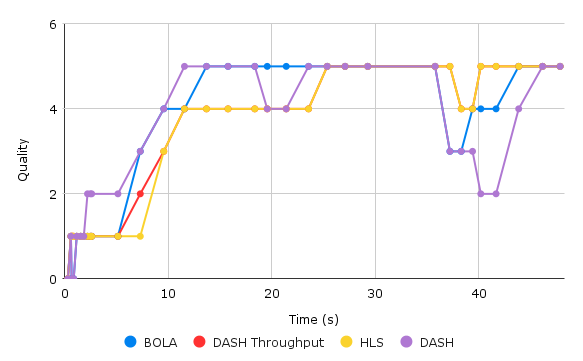
\includegraphics[width=\textwidth]{img/s1c1.png}
    \caption{Scenario 1. Quality vs time.}
    \label{fig:s1c1}
\end{figure}

\begin{figure}[]
    \centering
    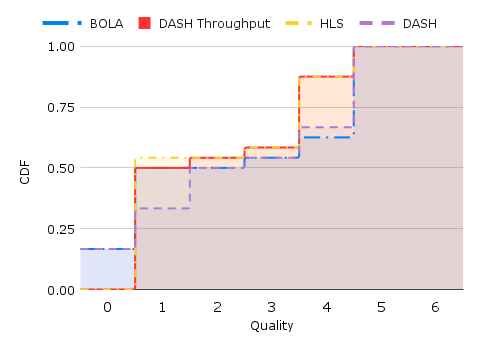
\includegraphics[width=\textwidth]{img/s1c2.png}
    \caption{Scenario 1. CDF quality.}
    \label{fig:s1c1}
\end{figure}


\subsection{Scenario 2}

\begin{figure}[]
    \centering
    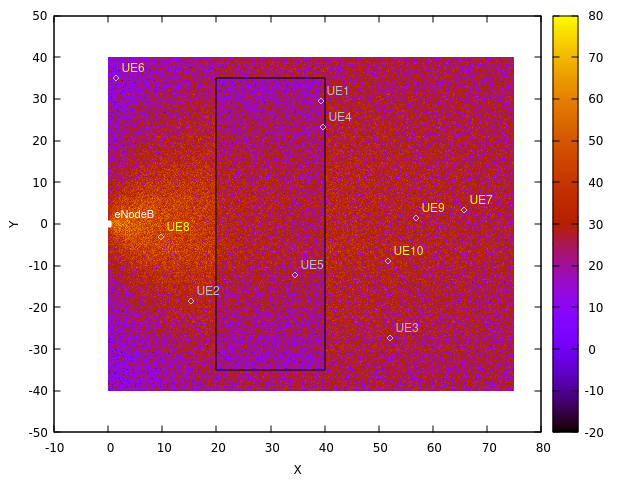
\includegraphics[width=\textwidth]{img/s2i1.png}
    \caption{Scenario 2. Radio Environment Map.}
    \label{fig:s1c1}
\end{figure}

\subsubsection{Good Conditions}


\subsubsection{Poor Conditions}


\subsection{Scenario 3}

Mixing applications


\section{Fairness}
\label{sec:fairness}

Fairness metrics are used to determine whether the adaptation 
algorithm is able to deliver an equitable share of the network bandwidth 
to different clients. In this analysis, the \textit{Jain Fairness Index (JFI)}
\cite{jfi} is used. The \textit{JFI} is calculated by this formula:

\begin{equation}
    JFI=\frac{\bigg(\sum\limits_{c\in C}\bar{B}\bigg)^2}{\left | C \right |\sum\limits_{c\in C}(\bar{B})^2}
\end{equation}

where  $C$ are the Clients and $\bar{B}$ are the Average Throughputs

\section{Conclusions}
\label{sec:simconclu}

limitations